\documentclass[12pt,a4paper,]{book}
\def\ifdoblecara{} %% set to true
\def\ifprincipal{} %% set to true
\let\ifprincipal\undefined %% set to false
\def\ifcitapandoc{} %% set to true
\let\ifcitapandoc\undefined %% set to false
\usepackage{lmodern}
% sin fontmathfamily
\usepackage{amssymb,amsmath}
\usepackage{ifxetex,ifluatex}
%\usepackage{fixltx2e} % provides \textsubscript %PLLC
\ifnum 0\ifxetex 1\fi\ifluatex 1\fi=0 % if pdftex
  \usepackage[T1]{fontenc}
  \usepackage[utf8]{inputenc}
\else % if luatex or xelatex
  \ifxetex
    \usepackage{mathspec}
  \else
    \usepackage{fontspec}
  \fi
  \defaultfontfeatures{Ligatures=TeX,Scale=MatchLowercase}
\fi
% use upquote if available, for straight quotes in verbatim environments
\IfFileExists{upquote.sty}{\usepackage{upquote}}{}
% use microtype if available
\IfFileExists{microtype.sty}{%
\usepackage{microtype}
\UseMicrotypeSet[protrusion]{basicmath} % disable protrusion for tt fonts
}{}
\usepackage[margin = 2.5cm]{geometry}
\usepackage{hyperref}
\hypersetup{unicode=true,
            pdfauthor={Nombre Completo Autor},
              pdfborder={0 0 0},
              breaklinks=true}
\urlstyle{same}  % don't use monospace font for urls
%
\usepackage[usenames,dvipsnames]{xcolor}  %new PLLC
\IfFileExists{parskip.sty}{%
\usepackage{parskip}
}{% else
\setlength{\parindent}{0pt}
\setlength{\parskip}{6pt plus 2pt minus 1pt}
}
\setlength{\emergencystretch}{3em}  % prevent overfull lines
\providecommand{\tightlist}{%
  \setlength{\itemsep}{0pt}\setlength{\parskip}{0pt}}
\setcounter{secnumdepth}{5}
% Redefines (sub)paragraphs to behave more like sections
\ifx\paragraph\undefined\else
\let\oldparagraph\paragraph
\renewcommand{\paragraph}[1]{\oldparagraph{#1}\mbox{}}
\fi
\ifx\subparagraph\undefined\else
\let\oldsubparagraph\subparagraph
\renewcommand{\subparagraph}[1]{\oldsubparagraph{#1}\mbox{}}
\fi

%%% Use protect on footnotes to avoid problems with footnotes in titles
\let\rmarkdownfootnote\footnote%
\def\footnote{\protect\rmarkdownfootnote}


  \title{}
    \author{Nombre Completo Autor}
      \date{18/11/2021}


%%%%%%% inicio: latex_preambulo.tex PLLC


%% UTILIZA CODIFICACIÓN UTF-8
%% MODIFICARLO CONVENIENTEMENTE PARA USARLO CON OTRAS CODIFICACIONES


%\usepackage[spanish,es-nodecimaldot,es-noshorthands]{babel}
\usepackage[spanish,es-nodecimaldot,es-noshorthands,es-tabla]{babel}
% Ver: es-tabla (en: https://osl.ugr.es/CTAN/macros/latex/contrib/babel-contrib/spanish/spanish.pdf)
% es-tabla (en: https://tex.stackexchange.com/questions/80443/change-the-word-table-in-table-captions)
\usepackage[spanish, plain, datebegin,sortcompress,nocomment,
noabstract]{flexbib}
 
\usepackage{float}
\usepackage{placeins}
\usepackage{fancyhdr}
% Solucion: ! LaTeX Error: Command \counterwithout already defined.
% https://tex.stackexchange.com/questions/425600/latex-error-command-counterwithout-already-defined
\let\counterwithout\relax
\let\counterwithin\relax
\usepackage{chngcntr}
%\usepackage{microtype}  %antes en template PLLC
\usepackage[utf8]{inputenc}
\usepackage[T1]{fontenc} % Usa codificación 8-bit que tiene 256 glyphs

%\usepackage[dvipsnames]{xcolor}
%\usepackage[usenames,dvipsnames]{xcolor}  %new
\usepackage{pdfpages}
%\usepackage{natbib}




% Para portada: latex_paginatitulo_mod_ST02.tex (inicio)
\usepackage{tikz}
\usepackage{epigraph}
\renewcommand\epigraphflush{flushright}
\renewcommand\epigraphsize{\normalsize}
\setlength\epigraphwidth{0.7\textwidth}

\definecolor{titlepagecolor}{cmyk}{1,.60,0,.40}

%\DeclareFixedFont{\titlefont}{T1}{ppl}{b}{it}{0.5in}

% \makeatletter
% \def\printauthor{%
%     {\large \@author}}
% \makeatother
% \author{%
%     Author 1 name \\
%     Department name \\
%     \texttt{email1@example.com}\vspace{20pt} \\
%     Author 2 name \\
%     Department name \\
%     \texttt{email2@example.com}
%     }

% The following code is borrowed from: https://tex.stackexchange.com/a/86310/10898

\newcommand\titlepagedecoration{%
\begin{tikzpicture}[remember picture,overlay,shorten >= -10pt]

\coordinate (aux1) at ([yshift=-15pt]current page.north east);
\coordinate (aux2) at ([yshift=-410pt]current page.north east);
\coordinate (aux3) at ([xshift=-4.5cm]current page.north east);
\coordinate (aux4) at ([yshift=-150pt]current page.north east);

\begin{scope}[titlepagecolor!40,line width=12pt,rounded corners=12pt]
\draw
  (aux1) -- coordinate (a)
  ++(225:5) --
  ++(-45:5.1) coordinate (b);
\draw[shorten <= -10pt]
  (aux3) --
  (a) --
  (aux1);
\draw[opacity=0.6,titlepagecolor,shorten <= -10pt]
  (b) --
  ++(225:2.2) --
  ++(-45:2.2);
\end{scope}
\draw[titlepagecolor,line width=8pt,rounded corners=8pt,shorten <= -10pt]
  (aux4) --
  ++(225:0.8) --
  ++(-45:0.8);
\begin{scope}[titlepagecolor!70,line width=6pt,rounded corners=8pt]
\draw[shorten <= -10pt]
  (aux2) --
  ++(225:3) coordinate[pos=0.45] (c) --
  ++(-45:3.1);
\draw
  (aux2) --
  (c) --
  ++(135:2.5) --
  ++(45:2.5) --
  ++(-45:2.5) coordinate[pos=0.3] (d);   
\draw 
  (d) -- +(45:1);
\end{scope}
\end{tikzpicture}%
}

% Para portada: latex_paginatitulo_mod_ST02.tex (fin)

% Para portada: latex_paginatitulo_mod_OV01.tex (inicio)
\usepackage{cpimod}
% Para portada: latex_paginatitulo_mod_OV01.tex (fin)

% Para portada: latex_paginatitulo_mod_OV03.tex (inicio)
\usepackage{KTHEEtitlepage}
% Para portada: latex_paginatitulo_mod_OV03.tex (fin)

\renewcommand{\contentsname}{Índice}
\renewcommand{\listfigurename}{Índice de figuras}
\renewcommand{\listtablename}{Índice de tablas}
\newcommand{\bcols}{}
\newcommand{\ecols}{}
\newcommand{\bcol}[1]{\begin{minipage}{#1\linewidth}}
\newcommand{\ecol}{\end{minipage}}
\newcommand{\balertblock}[1]{\begin{alertblock}{#1}}
\newcommand{\ealertblock}{\end{alertblock}}
\newcommand{\bitemize}{\begin{itemize}}
\newcommand{\eitemize}{\end{itemize}}
\newcommand{\benumerate}{\begin{enumerate}}
\newcommand{\eenumerate}{\end{enumerate}}
\newcommand{\saltopagina}{\newpage}
\newcommand{\bcenter}{\begin{center}}
\newcommand{\ecenter}{\end{center}}
\newcommand{\beproof}{\begin{proof}} %new
\newcommand{\eeproof}{\end{proof}} %new
%De: https://texblog.org/2007/11/07/headerfooter-in-latex-with-fancyhdr/
% \fancyhead
% E: Even page
% O: Odd page
% L: Left field
% C: Center field
% R: Right field
% H: Header
% F: Footer
%\fancyhead[CO,CE]{Resultados}

%OPCION 1
% \fancyhead[LE,RO]{\slshape \rightmark}
% \fancyhead[LO,RE]{\slshape \leftmark}
% \fancyfoot[C]{\thepage}
% \renewcommand{\headrulewidth}{0.4pt}
% \renewcommand{\footrulewidth}{0pt}

%OPCION 2
% \fancyhead[LE,RO]{\slshape \rightmark}
% \fancyfoot[LO,RE]{\slshape \leftmark}
% \fancyfoot[LE,RO]{\thepage}
% \renewcommand{\headrulewidth}{0.4pt}
% \renewcommand{\footrulewidth}{0.4pt}
%%%%%%%%%%
\usepackage{calc,amsfonts}
% Elimina la cabecera de páginas impares vacías al finalizar los capítulos
\usepackage{emptypage}
\makeatletter

%\definecolor{ocre}{RGB}{25,25,243} % Define el color azul (naranja) usado para resaltar algunas salidas
\definecolor{ocre}{RGB}{0,0,0} % Define el color a negro (aparece en los teoremas

%\usepackage{calc} 


%era if(csl-refs) con dolares
% metodobib: true


\usepackage{lipsum}

%\usepackage{tikz} % Requerido para dibujar formas personalizadas

%\usepackage{amsmath,amsthm,amssymb,amsfonts}
\usepackage{amsthm}


% Boxed/framed environments
\newtheoremstyle{ocrenumbox}% % Theorem style name
{0pt}% Space above
{0pt}% Space below
{\normalfont}% % Body font
{}% Indent amount
{\small\bf\sffamily\color{ocre}}% % Theorem head font
{\;}% Punctuation after theorem head
{0.25em}% Space after theorem head
{\small\sffamily\color{ocre}\thmname{#1}\nobreakspace\thmnumber{\@ifnotempty{#1}{}\@upn{#2}}% Theorem text (e.g. Theorem 2.1)
\thmnote{\nobreakspace\the\thm@notefont\sffamily\bfseries\color{black}---\nobreakspace#3.}} % Optional theorem note
\renewcommand{\qedsymbol}{$\blacksquare$}% Optional qed square

\newtheoremstyle{blacknumex}% Theorem style name
{5pt}% Space above
{5pt}% Space below
{\normalfont}% Body font
{} % Indent amount
{\small\bf\sffamily}% Theorem head font
{\;}% Punctuation after theorem head
{0.25em}% Space after theorem head
{\small\sffamily{\tiny\ensuremath{\blacksquare}}\nobreakspace\thmname{#1}\nobreakspace\thmnumber{\@ifnotempty{#1}{}\@upn{#2}}% Theorem text (e.g. Theorem 2.1)
\thmnote{\nobreakspace\the\thm@notefont\sffamily\bfseries---\nobreakspace#3.}}% Optional theorem note

\newtheoremstyle{blacknumbox} % Theorem style name
{0pt}% Space above
{0pt}% Space below
{\normalfont}% Body font
{}% Indent amount
{\small\bf\sffamily}% Theorem head font
{\;}% Punctuation after theorem head
{0.25em}% Space after theorem head
{\small\sffamily\thmname{#1}\nobreakspace\thmnumber{\@ifnotempty{#1}{}\@upn{#2}}% Theorem text (e.g. Theorem 2.1)
\thmnote{\nobreakspace\the\thm@notefont\sffamily\bfseries---\nobreakspace#3.}}% Optional theorem note

% Non-boxed/non-framed environments
\newtheoremstyle{ocrenum}% % Theorem style name
{5pt}% Space above
{5pt}% Space below
{\normalfont}% % Body font
{}% Indent amount
{\small\bf\sffamily\color{ocre}}% % Theorem head font
{\;}% Punctuation after theorem head
{0.25em}% Space after theorem head
{\small\sffamily\color{ocre}\thmname{#1}\nobreakspace\thmnumber{\@ifnotempty{#1}{}\@upn{#2}}% Theorem text (e.g. Theorem 2.1)
\thmnote{\nobreakspace\the\thm@notefont\sffamily\bfseries\color{black}---\nobreakspace#3.}} % Optional theorem note
\renewcommand{\qedsymbol}{$\blacksquare$}% Optional qed square
\makeatother



% Define el estilo texto theorem para cada tipo definido anteriormente
\newcounter{dummy} 
\numberwithin{dummy}{section}
\theoremstyle{ocrenumbox}
\newtheorem{theoremeT}[dummy]{Teorema}  % (Pedro: Theorem)
\newtheorem{problem}{Problema}[chapter]  % (Pedro: Problem)
\newtheorem{exerciseT}{Ejercicio}[chapter] % (Pedro: Exercise)
\theoremstyle{blacknumex}
\newtheorem{exampleT}{Ejemplo}[chapter] % (Pedro: Example)
\theoremstyle{blacknumbox}
\newtheorem{vocabulary}{Vocabulario}[chapter]  % (Pedro: Vocabulary)
\newtheorem{definitionT}{Definición}[section]  % (Pedro: Definition)
\newtheorem{corollaryT}[dummy]{Corolario}  % (Pedro: Corollary)
\theoremstyle{ocrenum}
\newtheorem{proposition}[dummy]{Proposición} % (Pedro: Proposition)


\usepackage[framemethod=default]{mdframed}



\newcommand{\intoo}[2]{\mathopen{]}#1\,;#2\mathclose{[}}
\newcommand{\ud}{\mathop{\mathrm{{}d}}\mathopen{}}
\newcommand{\intff}[2]{\mathopen{[}#1\,;#2\mathclose{]}}
\newtheorem{notation}{Notation}[chapter]


\mdfdefinestyle{exampledefault}{%
rightline=true,innerleftmargin=10,innerrightmargin=10,
frametitlerule=true,frametitlerulecolor=green,
frametitlebackgroundcolor=yellow,
frametitlerulewidth=2pt}


% Theorem box
\newmdenv[skipabove=7pt,
skipbelow=7pt,
backgroundcolor=black!5,
linecolor=ocre,
innerleftmargin=5pt,
innerrightmargin=5pt,
innertopmargin=10pt,%5pt
leftmargin=0cm,
rightmargin=0cm,
innerbottommargin=5pt]{tBox}

% Exercise box	  
\newmdenv[skipabove=7pt,
skipbelow=7pt,
rightline=false,
leftline=true,
topline=false,
bottomline=false,
backgroundcolor=ocre!10,
linecolor=ocre,
innerleftmargin=5pt,
innerrightmargin=5pt,
innertopmargin=10pt,%5pt
innerbottommargin=5pt,
leftmargin=0cm,
rightmargin=0cm,
linewidth=4pt]{eBox}	

% Definition box
\newmdenv[skipabove=7pt,
skipbelow=7pt,
rightline=false,
leftline=true,
topline=false,
bottomline=false,
linecolor=ocre,
innerleftmargin=5pt,
innerrightmargin=5pt,
innertopmargin=10pt,%0pt
leftmargin=0cm,
rightmargin=0cm,
linewidth=4pt,
innerbottommargin=0pt]{dBox}	

% Corollary box
\newmdenv[skipabove=7pt,
skipbelow=7pt,
rightline=false,
leftline=true,
topline=false,
bottomline=false,
linecolor=gray,
backgroundcolor=black!5,
innerleftmargin=5pt,
innerrightmargin=5pt,
innertopmargin=10pt,%5pt
leftmargin=0cm,
rightmargin=0cm,
linewidth=4pt,
innerbottommargin=5pt]{cBox}

% Crea un entorno para cada tipo de theorem y le asigna un estilo 
% con ayuda de las cajas coloreadas anteriores
\newenvironment{theorem}{\begin{tBox}\begin{theoremeT}}{\end{theoremeT}\end{tBox}}
\newenvironment{exercise}{\begin{eBox}\begin{exerciseT}}{\hfill{\color{ocre}\tiny\ensuremath{\blacksquare}}\end{exerciseT}\end{eBox}}				  
\newenvironment{definition}{\begin{dBox}\begin{definitionT}}{\end{definitionT}\end{dBox}}	
\newenvironment{example}{\begin{exampleT}}{\hfill{\tiny\ensuremath{\blacksquare}}\end{exampleT}}		
\newenvironment{corollary}{\begin{cBox}\begin{corollaryT}}{\end{corollaryT}\end{cBox}}	

%	ENVIRONMENT remark
\newenvironment{remark}{\par\vspace{10pt}\small 
% Espacio blanco vertical sobre la nota y tamaño de fuente menor
\begin{list}{}{
\leftmargin=35pt % Indentación sobre la izquierda
\rightmargin=25pt}\item\ignorespaces % Indentación sobre la derecha
\makebox[-2.5pt]{\begin{tikzpicture}[overlay]
\node[draw=ocre!60,line width=1pt,circle,fill=ocre!25,font=\sffamily\bfseries,inner sep=2pt,outer sep=0pt] at (-15pt,0pt){\textcolor{ocre}{N}}; \end{tikzpicture}} % R naranja en un círculo (Pedro)
\advance\baselineskip -1pt}{\end{list}\vskip5pt} 
% Espaciado de línea más estrecho y espacio en blanco después del comentario


\newenvironment{solutionExe}{\par\vspace{10pt}\small 
\begin{list}{}{
\leftmargin=35pt 
\rightmargin=25pt}\item\ignorespaces 
\makebox[-2.5pt]{\begin{tikzpicture}[overlay]
\node[draw=ocre!60,line width=1pt,circle,fill=ocre!25,font=\sffamily\bfseries,inner sep=2pt,outer sep=0pt] at (-15pt,0pt){\textcolor{ocre}{S}}; \end{tikzpicture}} 
\advance\baselineskip -1pt}{\end{list}\vskip5pt} 

\newenvironment{solutionExa}{\par\vspace{10pt}\small 
\begin{list}{}{
\leftmargin=35pt 
\rightmargin=25pt}\item\ignorespaces 
\makebox[-2.5pt]{\begin{tikzpicture}[overlay]
\node[draw=ocre!60,line width=1pt,circle,fill=ocre!55,font=\sffamily\bfseries,inner sep=2pt,outer sep=0pt] at (-15pt,0pt){\textcolor{ocre}{S}}; \end{tikzpicture}} 
\advance\baselineskip -1pt}{\end{list}\vskip5pt} 

\usepackage{tcolorbox}

\usetikzlibrary{trees}

\theoremstyle{ocrenum}
\newtheorem{solutionT}[dummy]{Solución}  % (Pedro: Corollary)
\newenvironment{solution}{\begin{cBox}\begin{solutionT}}{\end{solutionT}\end{cBox}}	


\newcommand{\tcolorboxsolucion}[2]{%
\begin{tcolorbox}[colback=green!5!white,colframe=green!75!black,title=#1] 
 #2
 %\tcblower  % pone una línea discontinua
\end{tcolorbox}
}% final definición comando

\newtcbox{\mybox}[1][green]{on line,
arc=0pt,outer arc=0pt,colback=#1!10!white,colframe=#1!50!black, boxsep=0pt,left=1pt,right=1pt,top=2pt,bottom=2pt, boxrule=0pt,bottomrule=1pt,toprule=1pt}



\mdfdefinestyle{exampledefault}{%
rightline=true,innerleftmargin=10,innerrightmargin=10,
frametitlerule=true,frametitlerulecolor=green,
frametitlebackgroundcolor=yellow,
frametitlerulewidth=2pt}





\newcommand{\betheorem}{\begin{theorem}}
\newcommand{\eetheorem}{\end{theorem}}
\newcommand{\bedefinition}{\begin{definition}}
\newcommand{\eedefinition}{\end{definition}}

\newcommand{\beremark}{\begin{remark}}
\newcommand{\eeremark}{\end{remark}}
\newcommand{\beexercise}{\begin{exercise}}
\newcommand{\eeexercise}{\end{exercise}}
\newcommand{\beexample}{\begin{example}}
\newcommand{\eeexample}{\end{example}}
\newcommand{\becorollary}{\begin{corollary}}
\newcommand{\eecorollary}{\end{corollary}}


\newcommand{\besolutionExe}{\begin{solutionExe}}
\newcommand{\eesolutionExe}{\end{solutionExe}}
\newcommand{\besolutionExa}{\begin{solutionExa}}
\newcommand{\eesolutionExa}{\end{solutionExa}}


%%%%%%%%


% Caja Salida Markdown
\newmdenv[skipabove=7pt,
skipbelow=7pt,
rightline=false,
leftline=true,
topline=false,
bottomline=false,
backgroundcolor=GreenYellow!10,
linecolor=GreenYellow!80,
innerleftmargin=5pt,
innerrightmargin=5pt,
innertopmargin=10pt,%5pt
innerbottommargin=5pt,
leftmargin=0cm,
rightmargin=0cm,
linewidth=4pt]{mBox}	

%% RMarkdown
\newenvironment{markdownsal}{\begin{mBox}}{\end{mBox}}	

\newcommand{\bmarkdownsal}{\begin{markdownsal}}
\newcommand{\emarkdownsal}{\end{markdownsal}}


\usepackage{array}
\usepackage{multirow}
\usepackage{wrapfig}
\usepackage{colortbl}
\usepackage{pdflscape}
\usepackage{tabu}
\usepackage{threeparttable}
\usepackage{subfig} %new
%\usepackage{booktabs,dcolumn,rotating,thumbpdf,longtable}
\usepackage{dcolumn,rotating}  %new
\usepackage[graphicx]{realboxes} %new de: https://stackoverflow.com/questions/51633434/prevent-pagebreak-in-kableextra-landscape-table

%define el interlineado vertical
%\renewcommand{\baselinestretch}{1.5}

%define etiqueta para las Tablas o Cuadros
%\renewcommand\spanishtablename{Tabla}

%%\bibliographystyle{plain} %new no necesario


%%%%%%%%%%%% PARA USO CON biblatex
% \DefineBibliographyStrings{english}{%
%   backrefpage = {ver pag.\adddot},%
%   backrefpages = {ver pags.\adddot}%
% }

% \DefineBibliographyStrings{spanish}{%
%   backrefpage = {ver pag.\adddot},%
%   backrefpages = {ver pags.\adddot}%
% }
% 
% \DeclareFieldFormat{pagerefformat}{\mkbibparens{{\color{red}\mkbibemph{#1}}}}
% \renewbibmacro*{pageref}{%
%   \iflistundef{pageref}
%     {}
%     {\printtext[pagerefformat]{%
%        \ifnumgreater{\value{pageref}}{1}
%          {\bibstring{backrefpages}\ppspace}
%          {\bibstring{backrefpage}\ppspace}%
%        \printlist[pageref][-\value{listtotal}]{pageref}}}}
% 
%%% de kableExtra
\usepackage{booktabs}
\usepackage{longtable}
%\usepackage{array}
%\usepackage{multirow}
%\usepackage{wrapfig}
%\usepackage{float}
%\usepackage{colortbl}
%\usepackage{pdflscape}
%\usepackage{tabu}
%\usepackage{threeparttable}
\usepackage{threeparttablex}
\usepackage[normalem]{ulem}
\usepackage{makecell}
%\usepackage{xcolor}

%%%%%%% fin: latex_preambulo.tex PLLC


\begin{document}

\bibliographystyle{flexbib}



\raggedbottom

\ifdefined\ifprincipal
\else
\setlength{\parindent}{1em}
\pagestyle{fancy}
\setcounter{tocdepth}{4}
\tableofcontents

\fi

\ifdefined\ifdoblecara
\fancyhead{}{}
\fancyhead[LE,RO]{\scriptsize\rightmark}
\fancyfoot[LO,RE]{\scriptsize\slshape \leftmark}
\fancyfoot[C]{}
\fancyfoot[LE,RO]{\footnotesize\thepage}
\else
\fancyhead{}{}
\fancyhead[RO]{\scriptsize\rightmark}
\fancyfoot[LO]{\scriptsize\slshape \leftmark}
\fancyfoot[C]{}
\fancyfoot[RO]{\footnotesize\thepage}
\fi

\renewcommand{\headrulewidth}{0.4pt}
\renewcommand{\footrulewidth}{0.4pt}

\hypertarget{construcciuxf3n-del-conjunto-de-datos}{%
\chapter{Construcción del conjunto de
datos}\label{construcciuxf3n-del-conjunto-de-datos}}

El primer paso a la hora de construir cualquier modelo de predicción es
disponer de datos adecuados que permitan explicar correctamente el
fenómeno en estudio, en este caso los incendios forestales en Andalucía.
Con este fin, se ha llevado a cabo un extenso estudio previo del dominio
del problema para conocer qué variables pueden ser relevantes de cara a
la predicción de incendios forestales, analizando estudios similares
realizados anteriormente así como otras fuentes relativas a la ecología
del fuego, que nos permitiesen conocer el efecto que cabría esperar de
estas variables.

Se ha querido adoptar un enfoque dinámico, es decir, el objetivo no es
construir un modelo estacionario que nos indique si una determinada zona
se verá afectada por un incendio forestal a lo largo de un amplio
periodo temporal, si no que se pretende ser capaz de predecir si un
determinado punto del territorio andaluz se verá afectado por un
incendio forestal en un momento concreto, en base a las covariables
correspondientes a ese lugar en ese momento. Es decir, se considera no
solo la dimensión espacial de los datos si no también la temporal, al
mayor nivel de desagregación disponible. Este es un enfoque mucho menos
explorado, debido fundamentalmente a dos factores:

\begin{enumerate}
\def\labelenumi{\arabic{enumi}.}
\tightlist
\item
  La dificultad de disponer de información fiable y de calidad
  desagregada espacio-temporalmente
\item
  La dificultad de trabajar con datos de estas características de cara
  al análisis y principalmente a la modelización, ya que son datos
  correlados en el tiempo y en el espacio.
\end{enumerate}

Queda claro, por tanto, que se trata de un problema complejo que
requiere de simplificaciones para poder ser abordado, más aun dadas las
limitaciones en los recursos computacionales disponibles y la enorme
cantidad de de datos que se están considerando y que requieren de un
procesamiento sumamente costoso desde un punto de vista computacional.

Por todo ello, esta sección es probablemente la de mayor importancia y
dificultad de todo el trabajo, ya que implica la toma de decisiones que
serán determinantes de cara al correcto desempeño de los modelos que se
construirán más adelante, requiere de un vasto conocimiento del problema
que permita un enfoque adecuado que haga posible la consecución de los
objetivos que se esperan conseguir, necesita del uso de técnicas
específicas de procesamiento de datos espaciales que no han sido
tratadas durante el grado y se ve fuertemente limitada por los escasos
recursos computacionales disponibles.

\hypertarget{determinaciuxf3n-del-marco-del-estudio}{%
\section{Determinación del marco del
estudio}\label{determinaciuxf3n-del-marco-del-estudio}}

El primer paso ha sido limitar el área y la franja temporal que abarcará
el estudio. Para ello, ha sido necesario basarse principalmente en la
disponibilidad y consistencia de la información requerida para el
proyecto y en las limitaciones computacionales impuestas por el equipo
disponible.

En cuanto a la disponibilidad de información, hay que diferenciar entre
la información de incendios forestales y la información de variables que
permitan explicar este fenómeno considerando la mayor desagregación
espacial y temporal posible.

\hypertarget{incendios-forestales}{%
\subsection{Incendios forestales}\label{incendios-forestales}}

En lo referente a los datos sobre incendios forestales cabe mencionar
que España cuenta con una de las mayores y más completas bases de datos
sobre incendios forestales a nivel europeo. Se trata de la Estadística
General de Incendios Forestales (EGIF), que en su versión definitiva
actualmente contiene toda la información que se recoge en cada parte de
incendio forestal que ha tenido lugar en España desde 1983 hasta 2015,
incluyendo su información espacial con sus coordenadas de origen. Se ha
explorado extensamente el uso de esta base de datos para el proyecto,
dada su exhaustividad y completitud. Sin embargo, lamentablemente no ha
sido posible en este caso incorporarla al trabajo por diversas razones.

La principal de ellas fue que hasta marzo de 2024 la base de datos de la
EGIF solo se encontraba disponible en el Catálogo de Datos del Gobierno
de España en formato TURTLE\footnote{TURTLE es una sintaxis para RDF con
  compatible con SPARQL. RDF (Resource Description Framework) es un
  estándar de semántica web utilizado para el intercambiar de datos en
  la Web.} y esto conllevó numerosas dificultades. Se exploraron
distintas librerías de R (y alguna de Python) para el manejo de datos en
este formato como RDFlib. Sin embargo, al tratarse de una base de datos
de un tamaño considerable (aproximadamente 1GB y con más de una decena
de millones de tripletas), esta librería no era suficientemente
eficiente para poder realizar consultas en un tiempo razonable al
conjunto de datos. Tras explorar otras alternativas, se valoró la
posibilidad de usar un triplestore, es decir, una base de datos
especialmente diseñada para el almacenamiento y recuperación de
tripletas a través de consultas semánticas. En este caso se usó Apache
Jena Fuseki, ya que cuenta con una interfaz que facilita su uso. Sin
embargo, aunque esto supuso una mejora considerable en la eficiencia y
permitió realizar consultas sencillas a la base de datos, en este caso
fue la complejidad del gráfico de datos (ontología) y la escasa
documentación disponible sobre esta, la que impidió que se pudiesen
realizar las consultas más complejas que requería para llevar a cabo el
proyecto. Además, se debe tener en cuenta que se trata de una base de
datos muy heterogénea y con numerosos datos faltantes debida su
naturaleza, por lo que requiere de un preprocesamiento que probablemente
será complicado y costoso en tiempo y en recursos computacionales. Al no
disponer de ninguno de estos, finalmente se optó por buscar una
alternativa más abarcable dada las limitaciones con las que cuenta un
Trabajo de Fin de Estudios, aunque queda abierta la posibilidad de
explorar esta base de datos en futuros estudios, la cual aportar nuevas
dimensiones al estudio de los incendios forestales en España gracias a
la enorme cantidad de información que ofrece.

Ante esta situación, la solución planteada fue limitar el área en
estudio a la Comunidad Autónoma de Andalucía, aprovechando la enorme
disponibilidad de información medioambiental que ofrece la Red de
Información Ambiental de Andalucía (REDIAM). En particular, se emplea la
cartografía generada por la REDIAM sobre las áreas recorridas por los
incendios forestales entre 1975 y 2022. Esta contiene los perímetros de
incendios forestales mayores de 100 ha en Andalucía obtenidos a partir
de imágenes de satélite y datos de campo. Se trata por tanto de una
información que no es exhaustiva, pues los incendios con una extensión
inferior a 100ha no han sido considerados. Sin embargo, frente a no
disponer de otra información operativa de mayor calidad, se utilizará
esta teniendo en cuenta que tendrá un efecto sobre las conclusiones que
se puedan sacar de los modelos que se construyan.

De esta forma, se han recopilado los polígonos de 1090 incendios
forestales ocurridos en Andalucía entre 2002 y 2022, junto con la fecha
de inicio de cada uno de ellos.

\hypertarget{variables-predictoras}{%
\subsection{Variables predictoras}\label{variables-predictoras}}

Una vez limitada la extensión territorial del estudio el siguiente paso
era acotar la franja temporal que abarcaría el estudio en base a la
disponibilidad de datos adecuados para explicar el fenómeno en cuestión
desagregados espacial y temporalmente.

Los incendios forestales son un proceso sumamente complejo, en el que
actúan numerosos factores de muy distinta índole (\ldots). Además,
dentro de un incendio forestal se pueden distinguir distintas fases que
presentan características muy diversas y sobre las que actúan distintos
agentes: ignición, propagación y extinción. Dada la información sobre
incendios forestales disponible, se está obligado a adoptar un enfoque
global, pues no se dispone de los puntos de ignición u origen de los
incendios forestales. El enfoque será, por tanto, intentar predecir si
una determinada localización se verá afectada por un incendio forestal
(de más de 100 ha) en un momento concreto.

Además, es importante tener en cuenta que existen factores estructurales
que tienen una influencia directa sobre los regímenes de incendios
forestales como son las tendencias de uso y explotación de los bosques,
la presencia de interfaz urbano forestal, los tipos y técnicas de
agricultura que se llevan a cabo, la presencia e intensidad del
pastoreo, los cambios en los usos de suelo e incluso conductas sociales
y tendencias demográficas diversas. Se trata de variables que cambian a
lo largo de periodos relativamente largos de tiempo y que muy
difícilmente pueden ser incluidos en los modelos, dada la falta de datos
sobre ellas, así como su carácter transversal. Por ello, se ha
considerado conveniente no extender en exceso el periodo de estudio,
reconocida la imposibilidad de incluir en el modelo todas las variables
que tienen un impacto relevante en la aparición de incendios y que son
cambiantes en el tiempo.

Todo ello hace necesario que el conjunto de datos utilizado contenga
información sobre todas las dimensiones (o al menos las principales) que
influyen en cualquiera de las fases de un incendio forestal. Es decir,
se deben incluir la dimensión antropogénica, la demográfica, la
hidrográficas, la topográfica, la meteorológica y la vegetación. Es
importante recalcar que siempre se hace referencia a datos geoespaciales
pues debe ser la información relativa al lugar (y al momento) del
incendio, con la dificultad posterior que esto supondrá.

Por último, es importante diferenciar entre características que se
considerarán estructurales (y por tanto invariantes a lo largo del
periodo de estudio) y aquellas que se considerarán variables en el
tiempo. Dentro de las primeras se encuentran todas las características
relacionadas con la topografía del terreno, las infraestructuras y los
usos del suelo, como por ejemplo el modelo de elevaciones, la
distribución de asentamientos de población, la red de carreteras y el
uso de suelo. Todas las demás variables de carácter demográfico,
meteorológico o de vegetación se considerarán, por tanto, desagregadas
temporalmente.

En base a todo lo mencionado y a la disponibilidad de información de
calidad de las categorías comentadas, se ha decidido limitar la franja
temporal del estudio a 20 años que van de 2002 a 2022, ambos inclusive.

\hypertarget{fuentes-de-datos}{%
\section{Fuentes de datos}\label{fuentes-de-datos}}

Como se ha comentado en la sección anterior, los datos sobre los
incendios forestales se han obtenido de los perímetros de incendios
forestales mayores de 100 ha en Andalucía entre 1975 y 2020 disponibles
la REDIAM. De cada incendio registrado se dispone de su fecha de inicio,
del área recorrida por el fuego y del municipio en el que originó, así
como de otras variables que dependen del año de la campaña y que no son
relevantes de cara a nuestro estudio.

Tomando como base estudios similares (\ldots) y partiendo de las 6
categorías ya mencionadas se han recopilado 23 conjuntos de datos de
distinto tipo que se usarán para explicar y predecir los incendios
forestales en Andalucía. Estos conjuntos se recogen en la Tabla
\ref{tab:fuentes}, donde también se indica la fuente de la que ha sido
obtenido cada uno de ellos, el tipo de datos que contiene (indicando su
resolución en el caso de los datos ráster) y la frecuencia de las
observaciones (o resolución temporal) en el caso de las variables
temporales. En realidad, el número de archivos de datos que se manejan
es mucho mayor, ya que por ejemplo para la variable NDVI se dispone de
un archivo tiff para cada mes del periodo de estudio, lo que añade
cierta complejidad al manejo de la información.

Es relevante la heterogeneidad de los datos recopilados, pues se dispone
tanto de datos tabulares como de datos espaciales y dentro de estos
últimos de datos vectoriales y datos ráster, con distintas resoluciones,
distintas frecuencias y distintos sistemas de referencia de coordenadas.
Esto hará que el procesamiento de estos datos hasta obtener datos
adecuados para el análisis estadístico sea costoso y que deban
utilizarse técnicas específicas de geocumputación.

Cabe también mencionar que se ha optado por el uso de datos
meteorológicos basados en modelos y en observaciones satelitares, en
lugar del uso de datos provenientes de estaciones meteorológicas. Si
bien la información de estaciones meteorológica puede ser más precisa,
la dificultad de disponer de datos consistentes y continuos en el tiempo
a lo largo del periodo de estudio de las variables meteorológicas
seleccionadas ha hecho que este enfoque no sea viable. En esta dirección
se ha explorado la API de la AEMET y algunos paquetes de R como
\texttt{climate}, sin llegar a resultados satisfactorios. Por otro lado,
el paquete \texttt{nasapower} permite la descarga de una gran cantidad
de variables meteorológicas con frecuencia diaria y con una resolución
de aproximadamente \(0.5 \times 0.625\) grados de latitud y longitud
(unos 50km). Si bien es cierto que no es lo ideal, es la única opción
que se ha considerado viable y de cara a la construcción de unos
primeros modelos aproximativos podría ser suficiente. Si quisiese
extenderse el estudio, sería conveniente profundizar en la búsqueda de
alternativas que permitan obtener información meteorológica de una mayor
calidad y detalle.

\begin{table}
\begin{threeparttable}[]
\resizebox{\textwidth}{!}{
\begin{tabular}{lllll}
\hline
\textbf{Categoría}     & \textbf{Datos}          & \textbf{Fuente}    & \textbf{Tipo de dato}       & \textbf{Frecuencia} \\ \hline
\multirow{4}{*}{Topográficas}   & Altitud                                                        & DERA\tnote{a}  & TIFF (100m)        & -          \\
                                & Orientación                                                    & REDIAM\tnote{b}     & TIFF (100m)        & -          \\
                                & Pendiente                                                      & REDIAM     & TIFF (100m)        & -          \\
                                & Curvatura                                                      & REDIAM     & TIFF (100m)        & -          \\ \hline
Vegetación                      & NDVI                                                           & REDIAM     & TIFF (250m)        & Mensual    \\ \hline
\multirow{7}{*}{Antropogénicas} & Uso de suelo                                                   & DERA       & Shapefile          & -          \\
                                & Red de carreteras                                              & DERA       & Shapefile          & -          \\
                                & Red de ferrocarril                                             & DERA       & Shapefile          & -          \\
                                & Línea eléctrica                                                & DERA       & Shapefile          & -          \\
                                & Espacio protegido                                              & DERA       & Shapefile          & -          \\
                                & Senderos / Vías Verde / Carriles Bici                          & DERA       & Shapefile          & -          \\
                                & Caminos / Vías Pecuarias                                       & DERA       & Shapefile          & -          \\ \hline
Demográficas                    & Población del municipio                                        & IECA\tnote{c}       & csv                & Anual      \\ \hline
Hidrográficas                   & Principales Ríos                                               & MAGRAMA\tnote{d}    & Shapefile          & -          \\ \hline
\multirow{6}{*}{Meteorológicas} & Precipitación (mm/day)                                         & NASA POWER\tnote{e} & df (0.5º x 0.625º) & Diaria     \\
                                & Temperatura a 2m sobre la superficie (º)                       & NASA POWER & df (0.5º x 0.625º) & Diaria     \\
                                & Humedad del suelo (\%)                                         & NASA POWER & df (0.5º x 0.625º) & Diaria     \\
                                & Dirección del viento a 10 metros sobre la superficie terrestre(º) & NASA POWER & df (0.5º x 0.625º) & Diaria     \\
                                & Humedad relativa a 2m sobre la superficie (\%)                 & NASA POWER & df (0.5º x 0.625º) & Diaria     \\
                                & Cantidad de precipitaciones (mm/day)                           & NASA POWER & dfdf (0.5º x 0.625º) & Diaria     \\ \hline
\footnotesize Fuente: Elaboración propia
\end{tabular}}
\begin{tablenotes}
\raggedright
\item[a] {\footnotesize \href{https://www.juntadeandalucia.es/institutodeestadisticaycartografia/dega/datos-espaciales-de-referencia-de-andalucia-dera/descarga-de-informacion}{Datos Espaciales de Referencia de Andalucía (DERA)}}
\item[b] {\footnotesize \href{https://portalrediam.cica.es/descargas?path=%2F}{Descargas Rediam}}%2F}{Descargas Rediam}}
\item[c] {\footnotesize \href{https://www.juntadeandalucia.es/institutodeestadisticaycartografia/dega/}{Instituto de Estadística y Cartografía de Andalucía (IECA)}}
\item[d] {\footnotesize Ministerio de Agricultura, Alimentación y Medio Ambiente (MAGRAMA)}
\item[e] {\footnotesize \href{https://power.larc.nasa.gov/#resources}{NASA Prediction Of Worlwide Energy Resources (NASA POWER)}}
\end{tablenotes}
\caption{Datos brutos}
\label{tab:fuentes}
\end{threeparttable}
\end{table}

\hypertarget{procesamiento-de-los-datos}{%
\section{Procesamiento de los datos}\label{procesamiento-de-los-datos}}

Una vez se dispone de todos los conjuntos de datos que se usarán en el
estudio, el siguiente paso será combinarlos de manera adecuada y
transformarlos a un formato apto para el análisis estadístico y la
construcción de modelos predictivos, es decir, a un data frame. Dado que
el objetivo que se persigue es predecir si, dada unas condiciones
meteorológicas concretas en un momento dado, un punto del territorio
andaluz se verá afectado o no por un incendio forestal, será necesario
disponer de una cantidad suficiente de muestras negativas y positivas
distribuidas espacial y temporalmente que tengan asociadas las variables
explicativas correspondientes.

Intuitivamente, las muestras positivas serán aquellas observaciones
(puntos definidos en el tiempo y en el espacio) dentro del marco
espacio-temporal del estudio en las que se ha detectado un incendio
forestal en el día de la observación. Es decir, son observaciones dentro
de los polígonos de incendios el día que estos se han producido. Por
tanto, las muestras negativas serán observaciones dentro del marco
espacio-temporal definido en las que no se ha detectado un incendio
forestal. Es imporante tener en cuenta que dado que solo se dispone de
los incendios con una extensión mayor a 100 ha, la muestra cuenta con un
importante sesgo, ya que los casos positivos están infrarepresentados.
Por ello, no podremos hacer inferencia a todos los incendios forestales,
si no solo a los de una extensión superior a 100ha.

A continuación se detalla el proceso seguido para generar el conjunto de
datos depurado sobre el que desarrollar el estudio a partir de los
distintos conjuntos de datos en bruto:

\begin{enumerate}
\def\labelenumi{\arabic{enumi}.}
\tightlist
\item
  Generación de una muestra balanceada de casos positivos y negativos.
\item
  Asignación de las variables descriptivas a cada observación.
\item
  Depuración de la muestra.
\end{enumerate}

\hypertarget{generaciuxf3n-de-una-muestra-balanceada-de-casos-positivos-y-negativos.}{%
\subsection{Generación de una muestra balanceada de casos positivos y
negativos.}\label{generaciuxf3n-de-una-muestra-balanceada-de-casos-positivos-y-negativos.}}

Para poder construir cualquier modelo de clasificación binaria se
necesita disponer de una muestra que cuente con un número suficiente de
casos positivos y negativo. Además, es aconsejable trabajar con
conjuntos de datos balanceados para evitar sesgos en los modelos de
clasificación {[}ARTICULO{]}.

Como ya se ha comentado, se considerarán observaciones positivas
aquellas que se hayan visto afectadas por un incendio forestal en el día
y lugar de la observación. En cambio, serán observaciones negativas
aquellas que no se hayan visto afectadas por un incendio forestal en el
día y lugar de la observación. Estas observaciones deberán generarse a
partir de los polígonos de incendios disponibles. Para ello, se usará un
enfoque similar al utilizado en
{[}\url{https://www.researchgate.net/publication/228527438_Learning_to_predict_forest_fires_with_different_data_mining_techniques}{]},
con algunas diferencias importantes. En {[}cita al paper{]} usan los
puntos de ignición como muestras positivas y su objetivo es predecir los
puntos de origen de los incendios forestales. En cambio, en el presente
trabajo no se disponen de los puntos de ignición de los incendios, por
lo que el enfoque adoptado es ligeramente diferente; el objetivo es
predecir las zonas que pueden verse afectadas por un incendio forestal
(superior a 100ha) bajo unas circunstancias concretas. De esta forma,
para construir la muestra de casos positivos se han generado 10 puntos
aleatorios dentro de cada polígono de incendio y se les ha asignado la
fecha del día de incio del incendio. Los casos negativos se generarán
igual que en {[}cita paper{]}: se toman fechas aleatorias dentro del
periodo de estudio y a cada una de ellas se le asocia una localización
aleatoria dentro del área de estudio satisfaciendo que deben estar a al
menos 15km de de cualquier incendio detectado en un margen de ± 3 días.
Esta forma de tomar los casos negativos asegura que estén lo
suficientemente alejados de los incendios forestales para representar
condiciones no influidas por estos, dando prioridad así a las áreas con
una menor prioridad de ocurrencia de incendio en un período definido.
Sin embargo, sería conveniente en estudios futuros plantearse si esos
parámetros (franja de ± 3 días y distancia superior a 15km) son
adecuados o tal vez sería más adecuado tomar otros valores, basados, por
ejemplo, en la duración media de los incendios en Andalucía y otras
características propias de los incendios en la región.

\begin{figure}[htb]
\centering
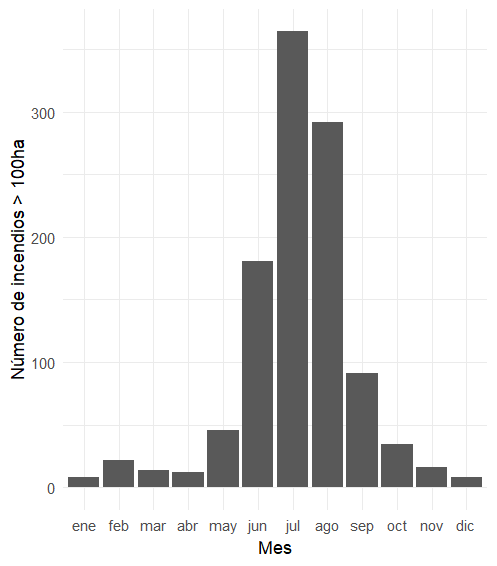
\includegraphics[width=0.5\textwidth]{graficos/incendios_mes.png}
\caption{Incendios durante el periodo de estudio}
\label{fig:incendios_mes}
\end{figure}

Tanto en (cita paper anterior) como en otros estudios consultados se
generan los casos negativos tomando fechas completamente aleatorias
dentro de la franja temporal del estudio. Sin embargo, esto induce un
claro sesgo en los datos, ya que las observaciones positivas no se
distribuyen uniformemente entre los 12 meses, si no que se concentran
marcadamente en los meses de verano, como puede observarse en la Figura
\ref{fig:incendios_mes}. Generar el conjunto de datos sin tener en
cuenta este hecho hace que las muestras positivas y negativas tengan
características meteorológicas muy diferenciadas que no responden al
verdadero proceso latente de aparición de incendios forestales sino al
proceso de selección de la muestra, pudiendo provocar un marcado sesgo
positivo en las medidas de evaluación de los modelos que en realidad no
estarían reflejando la realidad si no los sesgos introducidos en los
conjuntos de datos. Por ello, en el presente trabajo para de generar los
días de las muestras negativas se seguirá una distribución de
probabilidad proporcional a la cantidad de incendios observados a lo
largo del periodo de estudio en cada mes. Mediante este enfoque se
espera obtener una muestra balanceada y estratificada por mes que
permita construir modelos de clasificación capaces de captar los
patrones latentes de aparición de incendios forestales. Además, este
enfoque permite centrar el esfuerzo en los periodos que más incendios se
producen.

\hypertarget{asignaciuxf3n-de-las-variables-descriptivas-a-cada-observaciuxf3n}{%
\subsection{Asignación de las variables descriptivas a cada
observación}\label{asignaciuxf3n-de-las-variables-descriptivas-a-cada-observaciuxf3n}}

Una vez generada una muestra balanceada de 22170 observaciones dentro de
Andalucía entre el 1 de enero de 2002 y el 31 de diciembre de 2022, el
siguiente paso es asignar a cada una de ellas los valores
correspondientes a ese día y a esa localización concreta de todas las
variables predictoras a partir de los conjuntos de datos que se han
recopilado (recogidos en la Tabla \ref{tab:fuentes}). Dado que será
necesario calcular distancias, se usa un Sistema de Referencia de
Coordenadas proyectado al generar la muestra. En particular se usa una
variante del UTM30N por ser el que traen los archivos \emph{raster} de
las variables topográficas (es conveniente siempre que sea posible no
transformar el crs de los datos \emph{raster} pues al hacerlo se deben
interpolar los valores de los píxeles, produciendo pérdida de
información).

A continuación se detalla el proceso seguido para manipular construir
cada variable:

\begin{itemize}
\item
  Variables topográficas: Simplemente se extrae el dato del píxel en el
  que cae cada observación para cada uno de los conjuntos de datos.
\item
  Variables antropológicas:

  \begin{itemize}
  \item
    Se calculan las distancias de cada observación a la red de
    carreteras, a la red de ferrocarril, a las poblaciones y a la línea
    electrica, creando así las variables \emph{dist\_carreteras},
    \emph{dist\_ferrocarril}, \emph{dist\_poblaciones} y
    \emph{dist\_electr}, respectivamente. Las geometrías de los
    senderos, de las vías verdes y de los carriles bicis se unen y se
    calcula la distancia de cada observación a este conjunto de
    geometrías, generando así la variable \emph{dist\_sendero}. De la
    misma forma se procede con los caminos y las vías pecuarias, que dan
    origen a la variable \emph{dist\_camino}. Estas uniones se han
    llevado a cabo por considerar que sus elementos tienen
    características similares. Siempre se hace referencia a la distancia
    euclídea.
  \item
    Para construir una variable dicotómica \emph{enp} que indique si la
    observación se encuentra o no dentro de un Espacio Natural Protegido
    primero se ha rasterizado el conjunto de polígonos de Espacios
    Naturales Protegidos de Andalucía (de forma que en cada píxel se
    indica 1 si el centro de este está dentro del polígono de un ENP o 0
    si no) y posteriormente se ha extraído el valor del píxel que
    contiene a cada observación. En la rasterización se ha usado como
    modelo el ráster de eleviaciones con una resolución de
    \(100m \times 100m\). Proceder de este modo hace que se pierda algo
    de resolución pero resulta muchísimo más eficiente
    computacionalmente que comprobar para cada observación la relación
    espacial ``estar dentro del polígono de algún ENP'' (este enfoque
    resultaba computacionalmente inabarcable para el equipo disponible).
  \item
    Para construir la variable \emph{uso\_suelo} se ha procedido de
    manera similar. Primero se ha rasterizado, usando como modelo el
    mapa de elevaciones con una resolución de \(100m \times 100m\),
    asignando a cada píxel la categoría de uso de suelo del polígono que
    cubriese el centro del píxel. Y posteriormente, para cada
    observación se ha extraído el valor del píxel sobre el que
    estuviese. De nuevo, se ha procedido así por cuestiones de
    eficiencia. Es necesario hacer algunos comentarios más sobre esta
    variable. La información de uso de suelo proviene del mapa de
    Ocupación de Uso de Suelo CORINE Land Cover 2018, donde se
    establecen con 3 niveles de clasificación con 5, 15 y 44 clases,
    respectivamente. La primera clase se corresponde con el primer
    dígito del código, las segunda con el segundo y la tercera con el
    tercero. En este trabajo se ha decidido trabajar con el segundo
    nivel de clasificación. En la Tabla \ref{tab:codigos_uso_suelo} se
    recoge la clase correspondiente a cada código.
  \end{itemize}
\end{itemize}

\begin{table}[]
\resizebox{\columnwidth}{!}{%
\begin{tabular}{@{}lll@{}}
\toprule
Nivel 1                                                     & Nivel 2                                                  & Código \\ \midrule
Superficies artificiales                                    & Zonas urbanas                                            & 11     \\
                                                            & Zonas industriales, comerciales y de transporte          & 12     \\
                                                            & Zonas de extracción minera, vertederos y de construcción & 13     \\
                                                            & Zonas verdes artificiales, no agrícolas                  & 14     \\ \hline
Zonas agrícolas                                             & Tierras de labor                                         & 21     \\
                                                            & Cultivos permanentes                                     & 22     \\
                                                            & Prados y praderas                                        & 23     \\
                                                            & Zonas agrícolas heterogéneas                             & 24     \\ \hline
Zonas forestales con vegetación natural y espacios abiertos & Bosque                                                   & 31     \\ 
                                                            & Espacios de vegetación arbustiva y/o herbácea            & 32     \\
                                                            & Espacios abiertos con poca o sin vegetación              & 33     \\ \hline
Zonas húmedas                                               & Zonas húmedas continentales                              & 41     \\
                                                            & Zonas húmedas litorales                                  & 42     \\ \hline
Superficies de agua                                         & Aguas continentales                                      & 51     \\
                                                            & Aguas marinas                                            & 52     \\ \bottomrule
\end{tabular}%
}
\caption{Códigos de uso de suelo}
\label{tab:codigos_uso_suelo}
\end{table}

\begin{itemize}
\item
  Para construir la variable \emph{poblacion} se ha asignado a cada
  observación el código del municipio en el que está y se ha hecho un
  \emph{left\_join} con el código del municipio y el año de la
  observación. Para la variable \emph{dens\_población} se ha procedido
  de la misma manera pero se ha divido por la extensión del municipio en
  \(km^2\).
\item
  La distancia a los ríos \emph{dist\_rios} se ha obtenido simplemente
  calculando la distancia de cada observación al conjunto de geometrías
  de los principales ríos de España.
\item
  El NDVI viene en archivos \emph{raster} mensuales (lo que supone un
  total de unos 240 archivos en formato \emph{.tiff}). Para cada
  observación se ha extraído el valor del píxel correspondiente (en
  función de las coordenadas del punto) del archivo correspondiente (que
  depende del mes y año de la observación).
\end{itemize}

\hypertarget{depuraciuxf3n-de-la-muestra}{%
\subsection{Depuración de la
muestra}\label{depuraciuxf3n-de-la-muestra}}

Una vez construido el conjunto de datos ``en bruto'', se tratan los
valores perdidos y se ajustan adecuadamente los tipos de las variables.
En primer lugar se convierten en factores las variables \emph{fire},
\emph{enp} y \emph{uso\_suelo}. A continuación se codifican las
variables numéricas \emph{WD10M} y \emph{orientación} en los 4 puntos
cárdinales y sus bisectrices, generando así 8 clases (``N'', ``NW'',
``W'', ``SW'', ``S'', ``SE'', ``E'', ``NE''). En el caso de la variable
orientación se añade también la clase ``plano'', si la pendiente en ese
punto es 0.

El conjunto de datos construido tiene \(200\) registros incompletos, lo
cual supone un \(0.1\%\) del total de registros. De estos, el \(68\%\)
son casos negativos y el \(32\%\) son casos positivos. Los valores
perdidos se encuentran en las variables demográficas (85), en
\emph{uso\_suelo} (8), en NDVI (85) y en las variables topográficas
(53). Las causas de los datos perdidos faltantes son:

\begin{itemize}
\item
  El dato no está disponible para esa observación. Esto sucede con las
  variables demográficas (hay años para los que no está disponible el
  número de habitantes de algunos municipios) y el NDVI (para algunos
  meses no se dispone del archivo correspondiente).
\item
  En el caso de las variables topográficas los valores perdidos se
  encuentran todos en los límites de la comunidad (Figura
  \ref{fig:nas_topograficas}). Al proceder de datos en formato
  \emph{raster}, los píxeles con información no se ajustan exactamente a
  los límites de Andalucía (ya que son cuadrados). Esto provoca que para
  algunos puntos situados en los bordes del polígono no esté disponible
  la información de las variables topográficas.
\end{itemize}

Tras explorar otras alternativas y teniendo en cuenta tanto el reducido
número de registros incompletos como la naturaleza de los valores
desconocidos, se opta simplemente por eliminar estos registros.

\begin{figure}[htb]
\centering
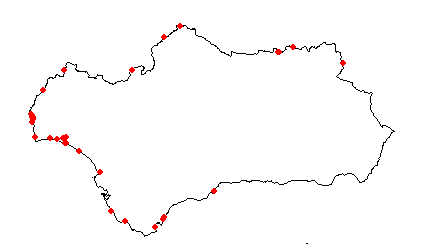
\includegraphics[width=0.5\textwidth]{graficos/nas_topograficas.png}
\caption{Observaciones para los que no está disponible alguna de las variables topográficas}
\label{fig:nas_topograficas}
\end{figure}

El resultado de todo este proceso es un conjunto de datos con 21546
registros y 27 variables, las cuales se detallan en la Tabla
\ref{tab:variables}.

\begin{table}[]
\resizebox{\columnwidth}{!}{%
\begin{tabular}{llll}
\hline

Categoría         & Nombre           & Descripción                                                                            & Tipo       \\ \hline
Topográficas      & elevacion        & Elevación sobre el nivel del mar (m)                                                   & numérica   \\
                  & orientacion      & Orientación de la pendiente descendiente                                               & categórica \\
                  & pendiente        & Pendiente del terreno (º)                                                              & numérica   \\
                  & curvatura        & Curvatura de la superfie                                                               & numérica   \\
Vegetación        & NDVI             & Índice de vegetación de diferencia normalizada                                         & numérica   \\
Antropogénicas    & uso\_suelo       & Clasificación del uso del suelo                                                        & categórica \\
                  & dist\_carretera  & Distancia a la carretera más cercana (m)                                               & numérica   \\
                  & dist\_ferocarril & Distancia a la vía de ferrocarril más cercana (m)                                      & numérica   \\
                  & dist\_electr     & Distancia a la línea electrica más cercana (m)                                         & numérica   \\
                  & enp              & Espacio Natural Protegido                                                              & categórica \\
                  & dist\_sendero    & Distancia a la vía verde, al carril bici o al sendero más cercano (m)                  & numérica   \\
                  & dist\_camino     & Distancia al camino o a la vía pecuaria más cercano (m)                                & numérica   \\
Demográficas      & poblacion        & Número de habitantes del municipio                                                     & numérica   \\
Hidrográficas     & dist\_rios       & Distancia al río más próximo (m)                                                       & numérica   \\
Meteorológicas &
  PRECTRORCORR &
  \begin{tabular}[c]{@{}l@{}}Promedio corregido del total de precipitaciones en la superficie \\ de la tierra en masa de agua (incluye el contenido de agua en la nieve) (mm/día)\end{tabular} &
  numérica \\
                  & T2M              & Temperatura promedio del aire a 2 metros sobre la superficie de la tierra (ºC)         & numérica   \\
                  & GWETTOP          & Porcentaje de humedad del suelo                                                        & numérica   \\
                  & WD10M            & Promedio de la dirección del viento a 10 metros sobre la superficie de la tierra       & categórica \\
                  & WS10M            & Promedio de la velocidad del viento a 10 metros sobre la superficie de la tierra (m/s) & numérica   \\
                  & RH2M             & Humedad relativa a 2 metros sobre la superficie de la tierra                           & numérica   \\ \hline
Variable Objetivo & fire             & Incendio forestal                                                                      & categórica \\ \hline
Identificadoras   & date             & Fecha de la observación                                                                & fecha      \\
                  & municipio        & Nombre del municipio                                                                   & texto      \\
                  & cod\_municipio   & Código del municipio                                                                   & texto      \\
                  & geometry         & Geometría de los puntos                                                                & sfc       
\end{tabular}%
}
\caption{Conjunto de datos depurados}
\label{tab:variables}
\end{table}

\bibliography{bib/library.bib,bib/paquetes.bib}


%


\end{document}
